\documentclass[floatfix,nofootinbib,superscriptaddress,fleqn,preprint]{revtex4-2}  
%\documentclass[aps,epsfig,tightlines,fleqn]{revtex4}
\usepackage[utf]{kotex}
\usepackage[HWP]{dhucs-interword}
\usepackage[dvips]{color}
\usepackage{graphicx}
\usepackage{bm}
%\usepackage{fancyhdr}
%\usepackage{dcolumn}
\usepackage{defcolor}
\usepackage{amsmath}
\usepackage{amsfonts}
\usepackage{amssymb}
\usepackage{amscd}
\usepackage{amsthm}
\usepackage[utf8]{inputenc}
 \usepackage{setspace}
%\pagestyle{fancy}

\begin{document}

\title{\Large 2022년 1학기 물리학 I: Quiz 18}
\author{김현철\footnote{Office: 5S-436D (면담시간 매주
    화요일-16:00$\sim$20:00)}} 
\email{hchkim@inha.ac.kr}
\affiliation{Hadron Theory Group, Department of Physics,
Inha University, Incheon 22212, Republic of Korea }
\date{Spring semester, 2022}


\vspace{1.cm}
\begin{abstract}
\noindent \textbf{ {\color{red}주의}: \color{blue} 단 한 번의 부정행위도 절대
  용납하지 않습니다. 적발 시, 학점은 F를 받게 됨은 물론이고,
  징계위원회에 회부합니다. One strike out임을 명심하세요.}\\
\\
문제는 다음 쪽부터 나옵니다.  \\ \\
{\bf Date:} 2022년 5월 11일 (수) 15:30-16:15
\\
{\bf 학번:} \hspace{4cm}
{\bf 이름:} 

\end{abstract}
\maketitle

\newpage
\noindent {\bf 문제 1. (40 pt)} 
불체가 좌우로 흔들리는 수평면에 놓여 있다. 수평면은 진동수 2.0 Hz로
단조화진동을 한다. 물체와 수평면 사이의 정지마찰계수는
0.50이다. 물체가 미끄러지지 않는 상태에서 단순조화진동의 최대진폭은
얼마인가? 
 \newpage

{\color{gray} [문제 풀이 쪽]}

\newpage

\noindent {\bf 문제 2. (60 pt)}
그림~\ref{fig:1}처럼 질량이 $0.200$ kg인 물체 1이 마찰이 없는 윗면에서
8.00 m/s의 속력으로 오른쪽으로 미끄러지다가 정지한 물체 2와
탄성충돌을 한다. 물체 2와 연결된 용수철의 용수철 상수는
$1208.5\,\mathrm{N/m}$이다(용수철은 충돌에 영향을 주지 않는다고 가정하자).
충돌 후에 물체 2는 주기 0.10 초로 단순조화진동을 하고 물체 1은
윗면에서 아랫면으로 높이 $h=4.90$ m를 떨어졌다. 이때 물체 1이 착륙한
거리는 얼마인가? 
\begin{figure}[ht]
  \centering
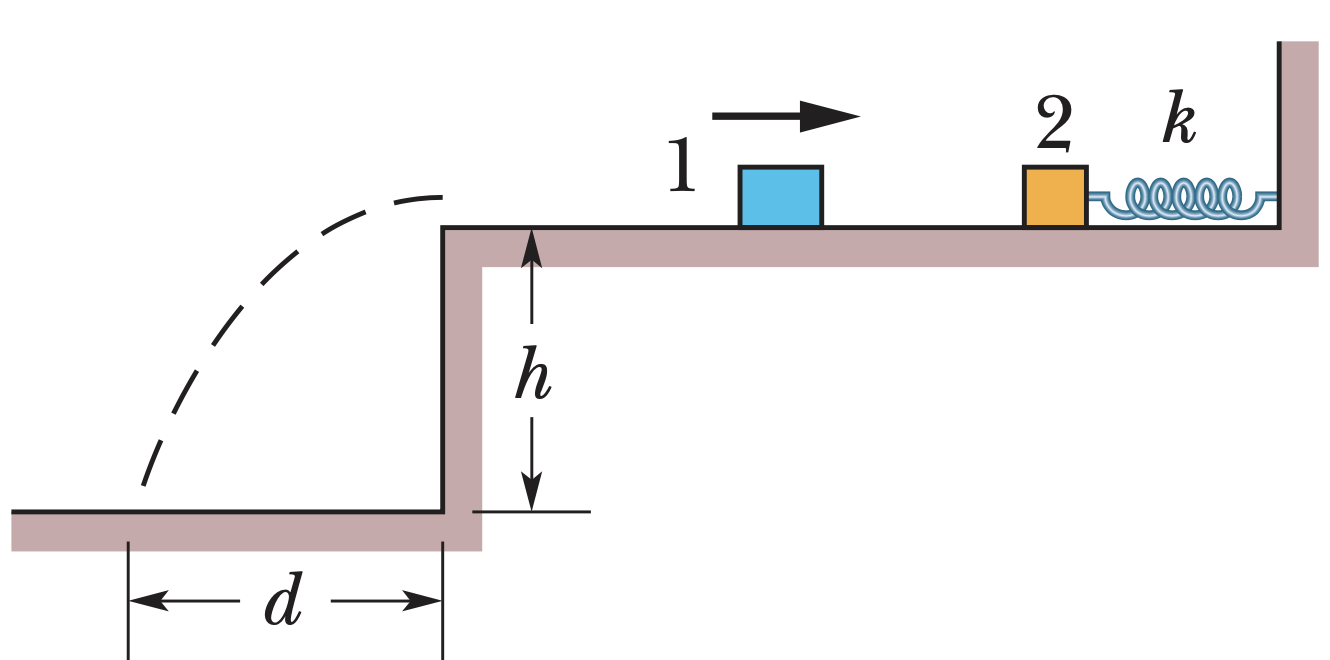
\includegraphics[scale=0.35]{Qfig18-1-20220511.png}
  \caption{문제 2}
  \label{fig:1}
\end{figure}

\newpage
{\color{gray} [문제 풀이 쪽]}

\newpage

\noindent {\bf 문제 3. (60pt)  }
그림~\ref{fig:2}처럼 길이가 $L=1.85$ m인 막대가 물리진자로 진동한다.
\begin{figure}[ht]
  \centering
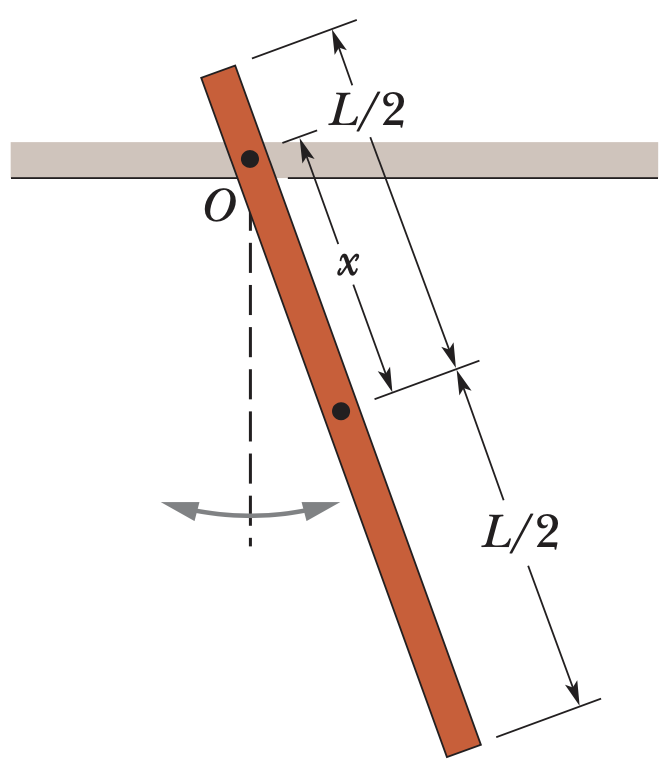
\includegraphics[scale=0.45]{Qfig18-2-20220511.png}
  \caption{문제 3}
  \label{fig:2}
\end{figure}
\begin{itemize}
\item[(가)] 막대의 중심질량과 회전축 사이의 거리 $x$가 얼마일 때
  주기가 최소이겠는가?
\item[(나)] 최소주기는 얼마인가?  
\end{itemize}
\newpage
{\color{gray} [문제 풀이 쪽]}

\newpage

\noindent {\bf 문제 4. (60pt)}
그림~\ref{fig:3}처럼 질량이 $M=5.4$ kg인 물체가 마찰이 없는 탁자
위에서 용수철상수 $k=6\,000\,\mathrm{N/m}$인 용수철에 달린 채 벽에
부착되어 있다. 질량은 $m=95$ g이고 속도 $\vec{v}$의 크기가 630 m/s인
총알이 날아가 물체 박혔다. 총알이 박힐 때까지 용수철의 압축은 무시할
정도라고 가정하면 충돌 직후에
\begin{figure}[ht]
  \centering
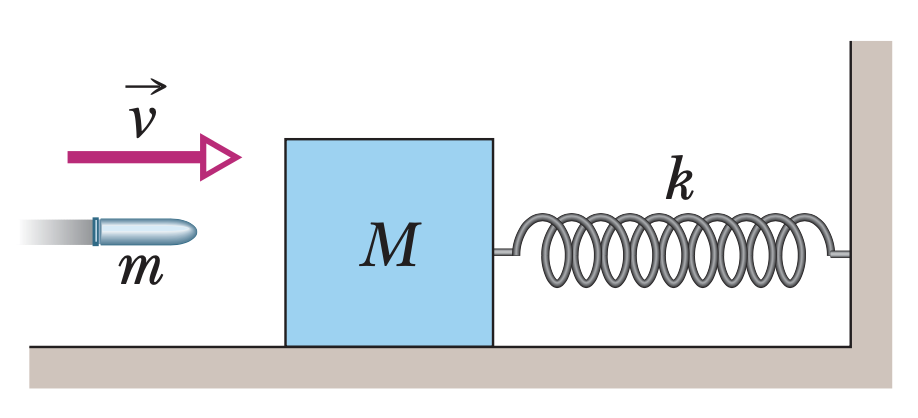
\includegraphics[scale=0.35]{Qfig18-3-20220511.png}
  \caption{문제 4}
  \label{fig:3}
\end{figure}
\begin{itemize}
\item[(가)] 물체의 속도와 
\item[(나)] 단순조화운동의 진폭은 각각 얼마인가?
\end{itemize}
\newpage
{\color{gray} [문제 풀이 쪽]}

\newpage
\end{document}